% !TeX root = ../../main.tex
% ##################################################################################################################
\section{Berlin I: BVG Scenario}
\label{ch:scenarios:berlinI}
\hfill \textbf{Author:} Andreas Neumann

% ##################################################################################################################
The Berliner Verkehrsbetriebe (BVG) is Berlin's main public transport company
and runs all kind of services with the exception of the S-Bahn urban rail
system. This includes bus services, the subway network, the largest tram network
of Germany as well as ferry services. The bus network consists of 149
different lines, 6468 directed stops and a vehicle fleet of 1316 buses \citep{BVG2012}.
In total, about 937~million trips were served by BVG in 2012,
41\,\% of them by bus.

% ------------
\createfigure%
{The city of Berlin and its transit network.}%
{The city of Berlin and its transit network.}%
{\label{fig:scenario_berlin_i}}%
{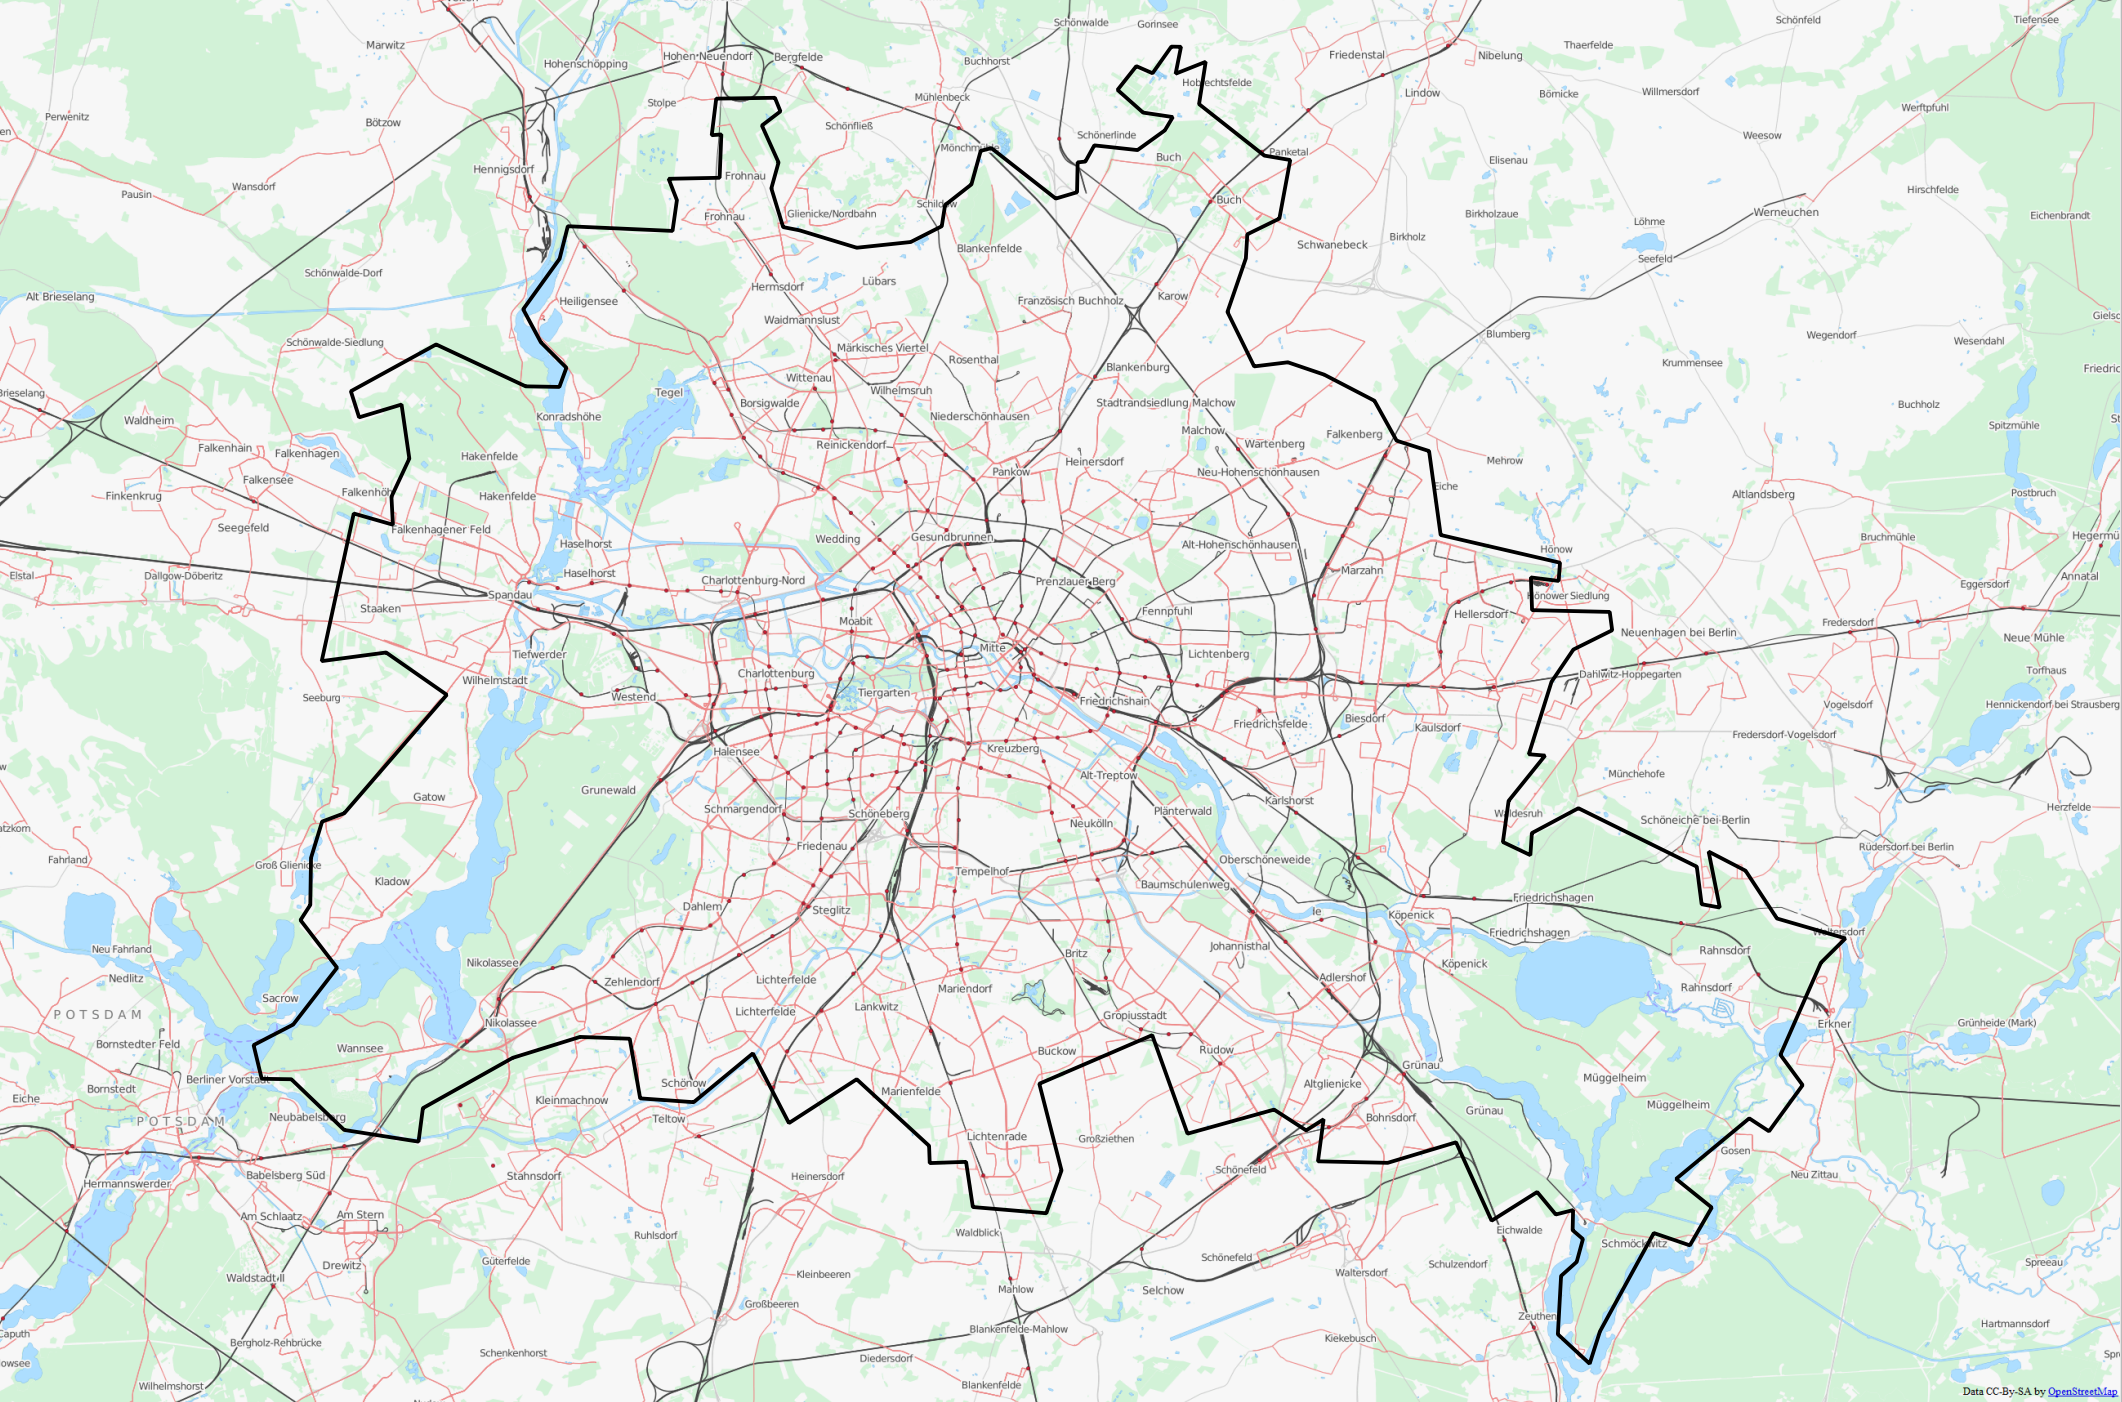
\includegraphics[width=0.99\textwidth, angle=0]{using/figures/berlin_pt}}%
{}
% ------------

% start excerpt from the paper
With the opening of the new international airport of Berlin and Brandenburg BER,
Berlin is expecting some major changes in travel demand. Especially, the
existing airport Tegel, currently exclusively served by buses operated by BVG,
will cease operations. BVG had thus a large interest in a new transport model
for the Berlin area. Due to the big changes, the model should not only deliver
the basis for future planning of the regional transport system, but has to
provide detailed information about passenger flows of different user groups as
well. Such user group specific analyses are considered of high importance for
the BVG in order to provide a basis for their future business strategies, which
is why an agent-based model was specifically requested. Two scenarios were
actually asked for, one for the year 2008 (actual state), and one for the year
2015 (prediction). To fulfill the needs mentioned above, the team of 
\citet{PTV2013}, \citet{Senozon2013} and \citet{VSP2013} at Technische Universit{\"a}t Berlin (TU Berlin)
offered a combined model consisting of both a static macroscopic model built with
PTV VISUM \citep{VISUM2013} as well as an integrated activity-based demand and
dynamic traffic assignment model built with MATSim. During
the project, attention was given that both models were based on the same data
sources and that both modeling processes interact with each other to allow data
exchange between the two models.
% end excerpt from the paper

In
brief, the model contains about 115,000 links, % 113269
about 15,000 directed stops, % 14902
6.0~million agents, % 4422012 (sex) 5992771 (/person)
and 539 public transport lines operated by BVG and other companies of the city
of Berlin and the state of Brandenburg. Among others the model features the transport modes Besides the transport modes car, For a more in-depth description of the
model, its generation and its calibration, the reader is referred to the work of
\cite{NeumannEtAl2014IatbrPtBerlinBook}. The model has been extensively been used in \citet[][Ch 7/8]{Neumann2014PhD} for the development of the minibus module of Section~\ref{sec:paratransit}.

% ##################################################################################################################
%\ah{
%\citep[][p.67ff]{Balmer_PhDThesis_2007}
%
%coupling with Visum BVG \\
%Marcel: IATBR \\
%}